\documentclass[11pt,a4paper]{ctexart}
\usepackage[utf8]{inputenc}
\usepackage{geometry}
\geometry{left=2.5cm,right=2.5cm,top=2.8cm,bottom=2.8cm}
\usepackage{amsmath,amssymb,amsfonts}
\usepackage{enumitem}
\usepackage{titlesec}
\usepackage{xcolor}
\usepackage{tcolorbox}
\usepackage{hyperref}

% 引入绝对位置放置宏包用于生成水印及插入图片宏包
\usepackage{graphicx}
\usepackage{eso-pic}



% --- 颜色定义 ---
\definecolor{mainblue}{RGB}{26, 82, 118}
\definecolor{secblue}{RGB}{41, 128, 185}
\definecolor{bglight}{RGB}{244, 246, 247}
\definecolor{textdark}{RGB}{44, 62, 80}

% --- 页面美化与字体设置 ---
\hypersetup{colorlinks=true, linkcolor=mainblue, urlcolor=secblue}
\setlist[itemize]{leftmargin=2em, itemsep=0.3em}
\setlist[enumerate]{leftmargin=2em, itemsep=0.3em}

% --- 标题样式自定义 ---
\titleformat{\section}{\large\bfseries\color{mainblue}}{\thesection}{1em}{}[{\color{mainblue}\titlerule[1pt]}]
\titleformat{\subsection}{\normalsize\bfseries\color{secblue}}{\thesubsection}{1em}{}
\titleformat{\subsubsection}{\small\bfseries\color{textdark}}{\thesubsubsection}{1em}{}

% --- 水印设置 (每页三个，斜45度，居中分布) ---
\newcommand{\WMText}{贺昱琪学习资料}
\newcommand{\WMScale}{2.28}
\newcommand{\WMAngle}{45}
\colorlet{WMColor}{black!8}

\AddToShipoutPictureBG{%
  \AtPageLowerLeft{%
    \put(\LenToUnit{0.66\paperwidth},\LenToUnit{0.70\paperheight}){%
      \rotatebox{\WMAngle}{\scalebox{\WMScale}{\textcolor{WMColor}{\WMText}}}%
    }%
    \put(\LenToUnit{0.33\paperwidth},\LenToUnit{0.50\paperheight}){%
      \rotatebox{\WMAngle}{\scalebox{\WMScale}{\textcolor{WMColor}{\WMText}}}%
    }%
    \put(\LenToUnit{0.66\paperwidth},\LenToUnit{0.30\paperheight}){%
      \rotatebox{\WMAngle}{\scalebox{\WMScale}{\textcolor{WMColor}{\WMText}}}%
    }%
  }%
}

\begin{document}

\begin{center}
    \LARGE \textbf{贺昱琪专项训练四}
\end{center}

\vspace{0.5cm}

\noindent \textbf{一、认真填一填（每小题 3 分，共 30 分）}

\begin{enumerate}
    \item 黑板上有 $1, 3, 5, 7, \dots$ 若干个连续奇数，小明擦掉其中一个，剩下的数的和为 2020，则小明擦掉的数为\underline{\hspace{2cm}}。\vspace{1.2cm}
    
    \item 一个两位数，十位上的数字与个位上的数字和是 9，把十位上的数字与个位上的数字对调后，得到的数与原数的比是 $4:5$，则原来的两位数是\underline{\hspace{2cm}}。\vspace{1.2cm}
    
    \item 已知等腰三角形一腰上的高和另一腰的夹角是 $25^\circ$，则这个等腰三角形的底角度数为\underline{\hspace{2cm}}。\vspace{1.2cm}
    
    \item 
    \begin{minipage}{0.65\textwidth}
        在长方形 ABCD 中，已知两邻边 AD=12，AB=5，对角线 AC=13，P 是 AD 边上异于 A 和 D 的一个动点，过点 P 分别向 OA，OD 作垂线 PE、PF，那么 $PE+PF$ 有\underline{\hspace{2cm}}值（最大、最小、定值），这个值为\underline{\hspace{2cm}}。
    \end{minipage}
    \hfill
    \begin{minipage}{0.3\textwidth}
        \centering
        
\includegraphics[width=\linewidth]{4.png}
    \end{minipage}
    \vspace{1.2cm}
    
    \item 
    \begin{minipage}{0.65\textwidth}
        如图，下列各三角形中的三个数之间均具有相同的规律，根据此规律，最后一个三角形中 $y$ 与 $n$ 之间的关系是\underline{\hspace{2cm}}。
    \end{minipage}
    \hfill
    \begin{minipage}{0.3\textwidth}
        \centering
        
\includegraphics[width=\linewidth]{5.png}
    \end{minipage}
    \vspace{1.2cm}
    
    \item 
    \begin{minipage}{0.65\textwidth}
        一个长 8 厘米，宽 7 厘米，高 6 厘米的长方体容器平放在桌面，里面盛有高 2 厘米的水（如图一）；将这个长方体沿着一条宽旋转 $90^\circ$，平放在桌面（如图二），水面的高度是\underline{\hspace{2cm}}。
    \end{minipage}
    \hfill
    \begin{minipage}{0.3\textwidth}
        \centering
        
\includegraphics[width=\linewidth]{6.png}
    \end{minipage}
    \vspace{1.2cm}
    
    \item 老师在黑板上写了若干个从 1 开始的连续自然数：$1, 2, 3, 4 \dots$，后来擦掉其中的一个，剩下的数的平均数是 $13\frac{9}{13}$，擦掉的自然数是\underline{\hspace{2cm}}。\vspace{1.2cm}
    
    \item 
    \begin{minipage}{0.65\textwidth}
        如图是圆柱被一个平面斜切后得到的几何体，请推算图中几何体的体积为\underline{\hspace{2cm}}。
    \end{minipage}
    \hfill
    \begin{minipage}{0.3\textwidth}
        \centering
        
\includegraphics[width=\linewidth]{8.png}
    \end{minipage}
    \vspace{1.2cm}
    
    \item 
    \begin{minipage}{0.65\textwidth}
        如图，E，G，F，H 分别为任意四边形 ABCD 的边 AD，AB，BC，CD 的中点，并且图中阴影部分的面积为 20 平方米，求图中四个小三角形的面积和，即 $S_1+S_2+S_3+S_4=$\underline{\hspace{2cm}}。
    \end{minipage}
    \hfill
    \begin{minipage}{0.3\textwidth}
        \centering
        
\includegraphics[width=\linewidth]{9.png}
    \end{minipage}
    \vspace{1.2cm}
    
    \item 某种数字化的信息传输中，先将信息转化为由数字 0 和 1 组成的数字串，并对数字串进行加密后再传输。现采用一种简单的加密方法：将原有的每个 1 都变成 10，原有的每个 0 都变成 01。我们用 $A_0$ 表示没有经过加密的数字串，这样对 $A_0$ 进行一次加密就得到一个新的数字串 $A_1$，对 $A_1$ 再进行一次加密又得到一个新的数字串 $A_2$，依此类推。例如 $A_0: 10$，则 $A_1: 1001$，若已知 $A_2: 100101101001$，则 $A_0$ 为\underline{\hspace{2cm}}；若数字串 $A_0$ 共有 4 个数字，则数字串 $A_4$ 中相邻两个数字相等的对数至少有\underline{\hspace{2cm}}对。\vspace{1.2cm}
\end{enumerate}

\vspace{0.8cm}

\noindent \textbf{二、细心算一算}

\begin{enumerate}
    \item[11.] 计算（每小题 4 分，共 16 分）
    \begin{enumerate}
        \item[(1)] $3.14 \times 4\frac{3}{10} + 31.4 \times 72\% - 0.314 \times 5$
        \vspace{3.5cm}
        
        \item[(2)] $55 \times \frac{1}{17} + 18\frac{1}{17} + 145 \times \frac{1}{11} \times \frac{11}{12}$
        \vspace{3.5cm}
        
        \item[(3)] $\left[ 1.65 \div 0.8 - \left(0.5 + \frac{1}{3}\right) \times \frac{24}{35} \right] \div \left(-\frac{3}{4} + \frac{1}{2}\right)$
        \vspace{3.5cm}
        
        \item[(4)] $\left( 1 + \frac{1}{2} + \frac{1}{3} + \dots + \frac{1}{2011} \right) \times \left( \frac{1}{2} + \frac{1}{3} + \dots + \frac{1}{2012} \right) - \left( 1 + \frac{1}{2} + \frac{1}{3} + \dots + \frac{1}{2012} \right) \times \left( \frac{1}{2} + \frac{1}{3} + \dots + \frac{1}{2011} \right)$
        \vspace{3.5cm}
    \end{enumerate}
\end{enumerate}

\vspace{0.8cm}

\noindent \textbf{三、用心想一想}

\begin{enumerate}
    \item[12.] (7分) 为了加强公民的节约意识，我市出台阶梯电价计算方案如下表：
    \begin{table}[htbp]
        \centering
        \begin{tabular}{|c|c|c|}
            \hline
            阶段 & 用电量范围 & 电价 \\
            \hline
            第一阶段 & 不超过 200 度的部分 & 0.50 元/度 \\
            \hline
            第二阶段 & 超过 200 度不超过 400 度的部分 & $a$ 元/度 \\
            \hline
            第三阶段 & 超过 400 度的部分 & 0.80 元/度 \\
            \hline
        \end{tabular}
    \end{table}
    \begin{enumerate}
        \item[(1)] 某户居民 2 月份应缴电费 78 元，该户 2 月份用电\underline{\hspace{2cm}}度；
        \vspace{1.5cm}
        \item[(2)] 某户居民 10 月份用电 220 度，缴电费 111 元，则 $a=$\underline{\hspace{2cm}}；
        \vspace{1.5cm}
        \item[(3)] 用 $x$ (度) 表示月用电量，请根据 $x$ 的不同取值范围用含 $x$ 的代数式表示该月应缴电费。
        \vspace{3.5cm}
    \end{enumerate}

    \item[13.] (8分) 某专卖店 5 月 1 日举行促销优惠活动，当天到该专卖店购买商品有两种方案：
    
    方案一：用 168 元购买会员卡成为会员后，凭会员卡购买店内任意商品，一律按商品价格的八折优惠；
    
    方案二：若不购买会员卡，则购买店内任何商品，一律按商品价格的九五折优惠。
    
    已知小芳 5 月 1 日前不是该店的会员。
    \begin{enumerate}
        \item[(1)] 若小芳不购买会员卡，购买一件商品时付了 380 元，她购买这件商品优惠多少元？
        \vspace{3.0cm}
        \item[(2)] 请你帮小芳算一算，当购买商品超过多少元时，采用方案一更合算？
        \vspace{3.5cm}
    \end{enumerate}

    \item[14.] (8分) 快、慢两车同时从甲、乙两地相向开出，快车行完全程需 10 小时，慢车行完全程需 15 小时，两车在途中相遇后，快车又行了 96 千米，这时快车已行了全程的 $\frac{4}{5}$。甲乙两地相距多少千米？
    \vspace{4.0cm}
    
    \item[15.] (9分) 将图所示的长方体石块 ($a > b > c$) 放入一圆柱形水槽内，并向水槽内匀速注水，速度为 $v \text{ cm}^3/\text{s}$，直至注满水槽为止。石块可以用三种不同的方式完全放入水槽内，如图1~图3所示。在这三种情况下，水槽内的水深 $h\text{cm}$ 与注水时间 $t\text{s}$ 的函数关系如图4~图6所示。根据图象完成下列问题：
    
    \begin{center}
        
\includegraphics[width=0.8\textwidth]{15.png}
    \end{center}
    
    \begin{enumerate}
        \item[(1)] 请分别将三种放置方式的示意图和与之对应的关系图象用线连接起来；
        \vspace{1.5cm}
        \item[(2)] 水槽的高\underline{\hspace{1.5cm}}cm；石块的长 $a=$\underline{\hspace{1.5cm}}cm；宽 $b=$\underline{\hspace{1.5cm}}cm；高 $c=$\underline{\hspace{1.5cm}}cm；
        \vspace{1.5cm}
        \item[(3)] 求圆柱形水槽的底面积 $S$。
        \vspace{3.5cm}
    \end{enumerate}
\end{enumerate}

\vspace{0.8cm}

\noindent \textbf{四、勇敢闯一闯}

\begin{enumerate}
    \item[16.] (10分) 一列火车出发 1 小时后因故停车 0.5 小时，然后以原速的 $\frac{3}{4}$ 前进，最终到达目的地晚 1.5 小时。若出发 1 小时后又前进 90 公里再因故停车 0.5 小时，然后同样以原速的 $\frac{3}{4}$ 前进，则到达目的地仅晚 1 小时。那么整个路程为多少公里？
    \vspace{4.5cm}

    \item[17.] (12分) 
    \begin{enumerate}
        \item[(1)] 如图 1 所示，已知正方形 ABCD 的边长为 $a$，$P$ 是边 CD 上一个动点（不与 C、D 重合），$CP=b$，以 CP 为一边在正方形 ABCD 的外部作正方形 PCEF，连接 BF、DF。\\
        ① 当 $a=4, b=2$ 时，四边形 ABFD 的面积为\underline{\hspace{2cm}}；\\
        ② 当 $a=4, b=3$ 时，四边形 ABFD 的面积为\underline{\hspace{2cm}}；\\
        观察计算：\\
        根据上述计算结果，你认为四边形 ABFD 的面积与正方形 ABCD 的面积之间有怎样的关系？请写出你的答案，并予以说明。
        \vspace{4.5cm}
        \item[(2)] 探索发现：\\
        如图 (2) 所示，连接 BD，若 $\triangle BDF$ 的面积为 12.5，正方形 PCEF 的面积为 4，点 M 是 BF 与 CD 的交点，求四边形 MCEF 的面积。
        \vspace{4.5cm}
    \end{enumerate}
    \begin{center}
        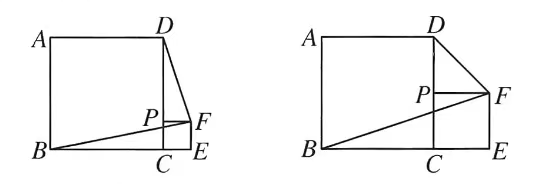
\includegraphics[width=0.6\textwidth]{17.png}
    \end{center}
\end{enumerate}

\end{document}